%%%%%%%%%%%%%%%%%%%%%%%%%%%%%%%%%%%%%%%%%
% Medium Length Professional CV
% LaTeX Template
% Version 2.0 (8/5/13)
%
% This template has been downloaded from:
% http://www.LaTeXTemplates.com
%
% Original author:
% Trey Hunner (http://www.treyhunner.com/)
%
% Important note:
% This template requires the resume.cls file to be in the same directory as the
% .tex file. The resume.cls file provides the resume style used for structuring the
% document.
%
%%%%%%%%%%%%%%%%%%%%%%%%%%%%%%%%%%%%%%%%%

%----------------------------------------------------------------------------------------
%	PACKAGES AND OTHER DOCUMENT CONFIGURATIONS
%----------------------------------------------------------------------------------------

\documentclass{resume} % Use the custom resume.cls style
\usepackage[dvipsnames]{xcolor}
\usepackage{gensymb}
\usepackage{graphicx}

\usepackage[left=0.75in,top=0.6in,right=0.75in,bottom=0.1in]{geometry} % Document margins
\newcommand{\tab}[1]{\hspace{.2667\textwidth}\rlap{#1}}
\newcommand{\itab}[1]{\hspace{0em}\rlap{#1}}
\name{Jeremy K. Thaller} % Your name
\address{10 Knowlton Dr. \\ Acton, MA 01720 \\ github: jthaller} % Your address
%\address{123 Pleasant Lane \\ City, State 12345} % Your secondary addess (optional)
%\address{github: jthaller \\ }
\address{+1 978-496-7990 \\ jkt2@alumni.williams.edu} % Your phone number and email
%\definecolor{darkpurple}{RGB}{108,48,130}

\renewenvironment{rSection}[1]{
	\sectionskip
	\textcolor{RoyalPurple}{\MakeUppercase{#1}}
	\sectionlineskip
	\hrule
	\begin{list}{}{
			\setlength{\leftmargin}{1.5em}
		}
		\item[]
	}{
	\end{list}
}

\begin{document}


%\begin{flushright}
%	\vspace{-3cm}
%	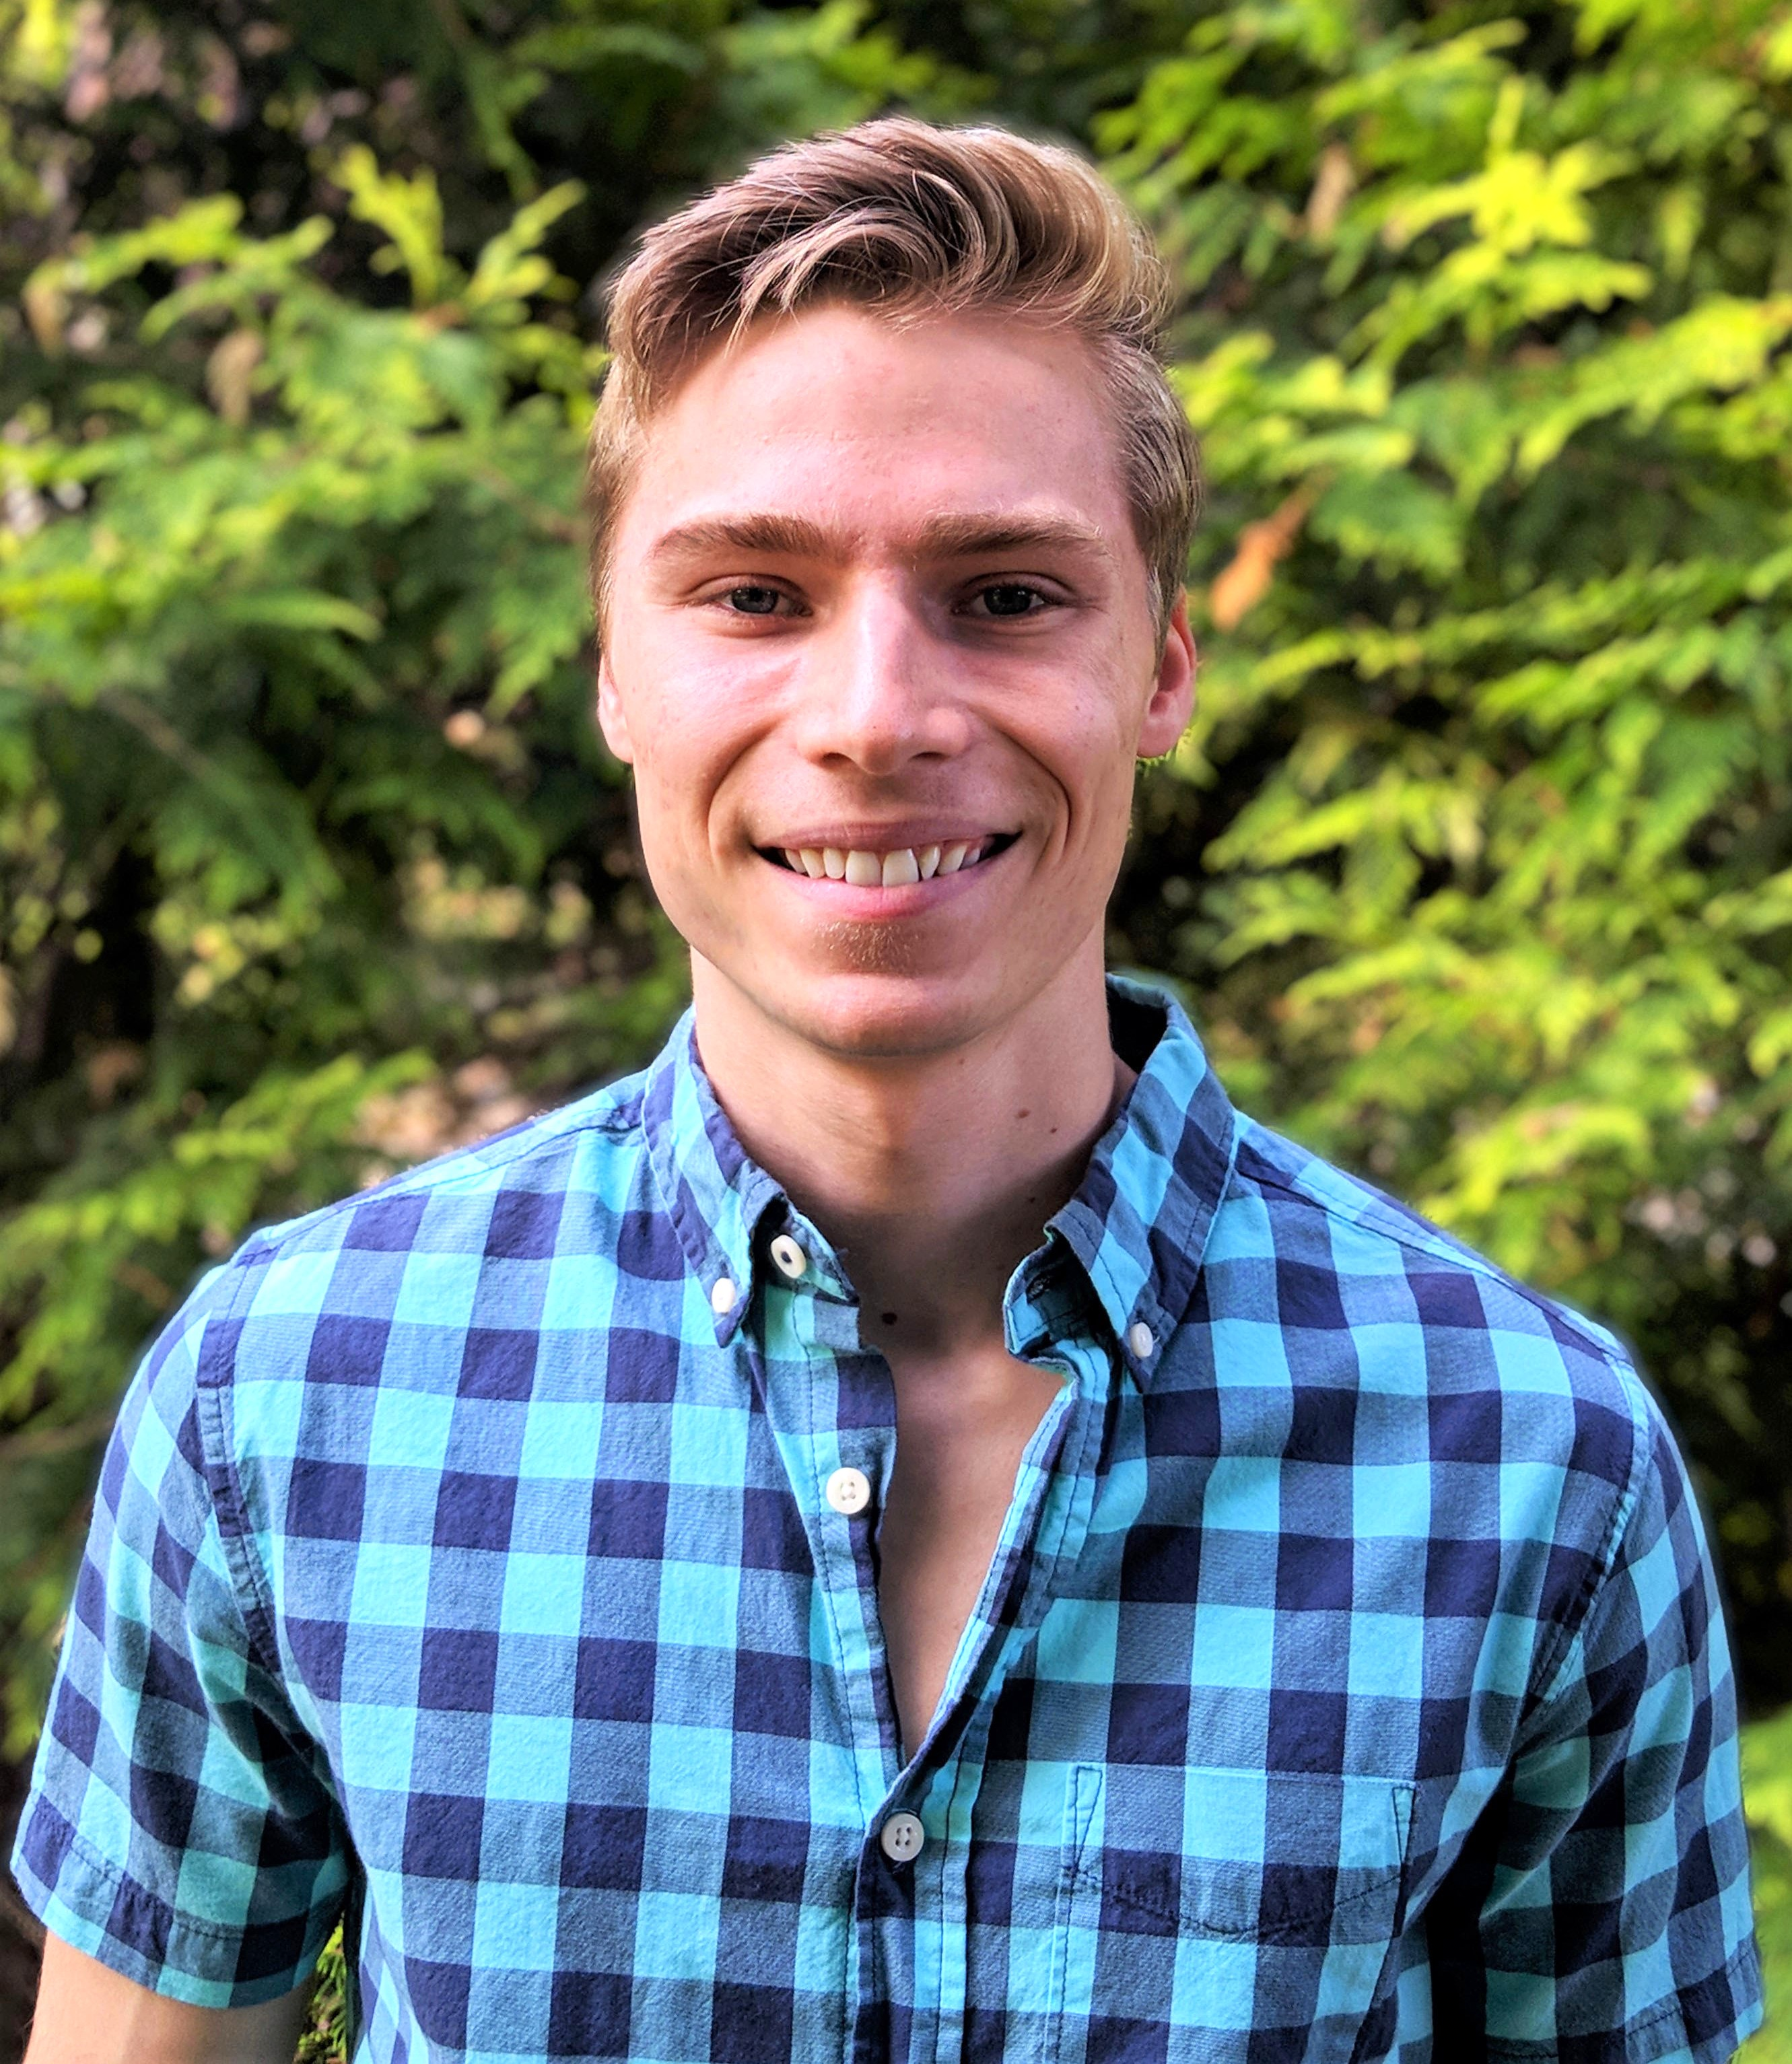
\includegraphics[width=3cm]{Jeremy_headshot_cropped.jpg}
%	\vspace{-1cm}
%\end{flushright}


	%----------------------------------------------------------------------------------------
	%	EDUCATION SECTION
	%----------------------------------------------------------------------------------------
\vspace{-2em}
	\begin{rSection}{Education} 
		\begin{rSubsection}{Ludwig Maximilians Universit{\"a}t  M{\"u}nchen (LMU) \&\\Technische Universit{\"a}t M{\"u}nchen (TUM)}{\em Oct. 2019 -- Present}{}{}
			\vspace{-.5em}
%			\item (In progress) MSci in Geophysics and Applied Physics (Joint Degree)
			\item (In progress) MSci in Geomaterials and Geochemistry
			\item Erasmus Mundus: Masters in Materials Science Exploring Large Scale Facilities
		\end{rSubsection}

%	{\bf Ludwig Maximilians Universit{\"a}t  M{\"u}nchen (LMU) \&\\Technische Universit{\"a}t M{\"u}nchen (TUM)} \hfill {\em Oct. 2019 -- Present}
%		\\Anticipated MSci in Geophysics and Applied Physics (Joint Degree)
%		\\Erasmus Mundus: Masters in Materials Science Exploring Large Scale Facilities
%
%		{\bf Williams College} \hfill {\em 2015 -- 2019}
%\\B.A. in Physics with Honors\\
%Pre-engineering Studies \hfill
%
%{\bf Acton-Boxborough Regional High School} \hfill {\em 2011 -- 2015}
%\\ National AP Scholar \hfill
%\\ National Honors Society
		\begin{rSubsection}{Williams College}{\em 2015 -- 2019}{}{}
			\vspace{-.5em}
			\item B.A. in Physics with Honors
			\item Pre-engineering Studies
			\item Sigma Xi
		\end{rSubsection}

		\begin{rSubsection}{Acton-Boxborough Regional High School}{\em 2011 -- 2015}{}{}
			\vspace{-.5em}
			\item National AP Scholar
			\item National Honors Society
		\end{rSubsection}



	\end{rSection}
	%----------------------------------------------------------------------------------------
	%	TECHNICAL STRENGTHS SECTION
	%----------------------------------------------------------------------------------------
	\newcommand{\CC}{C\nolinebreak\hspace{-.05em}\raisebox{.4ex}{\tiny\bf +}\nolinebreak\hspace{-.10em}\raisebox{.4ex}{\tiny\bf +}}
	\def\CC{{C\nolinebreak[4]\hspace{-.05em}\raisebox{.4ex}{\tiny\bf ++}}}

	\begin{rSection}{Technical Strengths}

		\begin{tabular}{ @{} >{\bfseries}l @{\hspace{6ex}} l }
			Programming Languages &  MATLAB, Python, JAVA, HTML, Arduino (C/\CC) \\
			Python Packages & Pandas, sklearn, KERAS, NumPy, Seaborn \\
			Data Software & Mathematica, Quantum Espresso, Excel, LabView, LoggerPro \\
			Other Software & LaTeX, Solid Works, VESTA, Adobe Illustrator, Adobe Photoshop   \\
			Machining Experience & Bridgeport Milling, CNC Milling, 3D Printing, Laser Cutting, \\ & Arc Melting, Fluorescent Confocal Microscopy, SEM, TEM, XRD
		\end{tabular}

	\end{rSection}

	%----------------------------------------------------------------------------------------
	%	RESEARCH EXPERIENCE SECTION
	%----------------------------------------------------------------------------------------

\vspace{-1em}
	\begin{rSection}{Research Experience}
		\begin{rSubsection}{Amorphous Solids, Metallic Glasses, \& Metallurgy}{Summer 2019}{Postbac Researcher}{}
			\vspace{-.5em}
			\item[] {\em Advised by Jan Schroers, Professor of Physics}\hfill {\em Yale University}
			\item Nanomolded crystalline metals to determine the underlying mechanism.
			\item Measured atomic surface properties with SEM and determined crystal orientation with TEM
		\end{rSubsection}


		\begin{rSubsection}{Soft Condensed Matter Physics}{May 2018 -- June 2019}{Undergraduate Honors Thesis}{}
			\vspace{-.5em}
				\item[] {\em Advised by Katharine E. Jensen, Professor of Physics}\hfill {\em Williams College}
				\item Designed and built stretching apparatus to induce equibiaxial stretch in soft materials
				\item Collect data via Fluorescent Confocal Microscopy 
				\item Data was analyzed through modified MATLAB scripts to measure the strain dependency of solid surface stress in soft materials via adhesion

		\end{rSubsection}
%
		%----------------------------------------------------------------------------


		\begin{rSubsection}{Atomic, Molecular, and Optical Physics}{Summer 2017}{Undergraduate Research Assistant}{}
			\vspace{-.5em}
			\item[] {\em Advised by Protik K. Majumder, Professor of Physics}\hfill {\em Williams College}
			\item Took data towards an ultra-precise  measurement of the Electric Quadrupole (E2) amplitude within the $6S^26P^2$ $^3P_0$ $\rightarrow$ $^3P_2$ transition in Pb
			\item Programed a PID controller in LabView to thermally regulate an oven to within $\pm .4\degree$ C at temperatures around $ 950\degree $ C
			\item Designed a deposition-rate detector for an indium cell chamber based on the mass dependent frequency of Quartz Crystals
		\end{rSubsection}

\end{rSection}

%------------------------------------------------------------------------------------
%       Data Science Skills
%------------------------------------------------------------------------------------
\begin{rSection}{Data Science Skills} \itemsep -2pt
	{Python} \\
	{Pandas}  \\
	{NumPy}  \\
	{Data Visualization} \\
	{Data Cleaning and Feature Engineering} \\
	{Command Line (BASH)} \\ 
	{SSH + EMACS} \\
	{Git and Version Control} \\
	{Probability and Statistics}
	
\end{rSection}

%------------------------------------------------------------------------------------
%       Teaching EXPERIENCE
%------------------------------------------------------------------------------------

\begin{rSection}{Teaching Experience} \itemsep -2pt
		\begin{rSubsection}{Math and Science Resource Center Tutor}{}{}{Williams College}{}
		\item {Tutored all introductory physics and calculus courses} \hfill {Spring 2019}
	\end{rSubsection}
	\begin{rSubsection}{Physics/Math TA}{}{}{Williams College}{}
		\item {Introduction to Mechanics}\hfill{Fall 2017 \& 2018}
		\item {Mathematical Methods for Scientists} \hfill {Spring 2018}
		\end{rSubsection}
	\begin{rSubsection}{Music Conducting}{}{}{UMASS Amherst}{}
		\item {George N. Parks Drum Major Academy staff member} \hfill {Summer 2015}
	\end{rSubsection}
\end{rSection}


%------------------------------------------------------------------------------------
%       WORK EXPERIENCE
%------------------------------------------------------------------------------------
\begin{rSection}{Other Work Experience} \itemsep -2pt
	\begin{rSubsection}{Office of Information Technologies}{June 2017 -- Aug. 2017}{}{Williams College}{}
	\item {Student Technology Assistant} \hfill {\em 40 hr/week}
	\end{rSubsection}
%-----------------------------
	\begin{rSubsection}{Williams College Wind Ensemble}{Sept. 2016 -- June 2017}{}{Williams College}{}
	\item {Teaching Assistant, Bassoonist} \hfill {\em 40 hr/week}
	\end{rSubsection}

\end{rSection}

%------------------------------------------------------------------------------------
%       Professional Memberships
%------------------------------------------------------------------------------------
	\begin{rSection}{Professional Memberships} \itemsep -2pt
		{Sigma Xi Associate Member} \hfill {June 2019 -- Present}\\
		{American Physical Society} \hfill {July 2018 -- Present}
		\\
		{New England Complex Fluids Workgroup} \hfill {May 2018 -- Present}

	\end{rSection}

%------------------------------------------------------------------------------------
%       Leadership
%------------------------------------------------------------------------------------
		\begin{rSection}{Leadership} \itemsep -2pt
		{Williams College Track Captain} \hfill {2018 -- 2019} \\
		{WASA (College Rocketry Club) Founder/President} \hfill {2017 -- 2019} \\
		{High School Track Captain} \hfill {2014 -- 2015}  \\
		{High School Head Drum Major} \hfill {2013 -- 2015}

	\end{rSection}



	%	EXAMPLE SECTION
	%----------------------------------------------------------------------------------------
%
%	\begin{rSection}{Achievements} \itemsep -2pt
%		{Michigan Institute for Computational Discovery Fellow }\hfill {\em Spring 2015} \\
%		{NSF GROW Fellowship Awardee}\hfill {\em Spring 2015} \\
%		{Community Coordinated Modeling Center Research Winner} \hfill {\em Spring 2015} \\
%		{NSF Graduate Research Fellowship Program Fellow}\hfill {\em Spring 2014}\\
%		{Rackham Merit Fellow}\hfill {\em Fall 2013}\\
%		{Template Developer for LaTeX} \hfill {\em September 2013 - Present} \\
%		{Backpacker and Hiking Enthusiast - have climbed 7 $>$ 14,000 ft peaks}
%	\end{rSection}




%------------------------------------------------------------------------------------
%       Publications
%------------------------------------------------------------------------------------
\begin{rSection}{Publications} \itemsep -2pt
	\item {Toward and Adhesion Based Measurement of Strain-Dependent}\hfill {\em Undergraduate Thesis}\\ Surface Stress in Soft Solids
\end{rSection}

%------------------------------------------------------------------------------------
%       Posters and Presentations
%--------------------------------------------------------------------------------
\pagebreak
\begin{rSection}{Posters and Presentations} \itemsep -2pt
%		\item {Toward and Adhesion Based Measurement of Strain-Dependent}\hfill {\em Williams Thesis Defense 2019}\\ Surface Stress in Soft Solids
%
%		\item {Adhesion-Based Measurements of Strain-Dependent \hfill {\em APS March Meeting 2019} \\Surface Stress in Soft Solids}
%
%		\item {Sprinkling stuff and then stretching it: How hard could it be?} \hfill {\em Williams Physics Thesis Update}
%
%		\item { Measuring Strain-Dependent Surface Stress in Soft Matter via Adhesion} \hfill {\em UMASS Soft Matter Day}
%
%		\item { A Precise Measurement of the Electric Quadrupole \hfill {\em Williams Summer Science 2017} \\ Amplitude Within the ${6S^2 6P^2}$ \space ${^3 P_0 \space \rightarrow} \space$ ${^3P_2}$ Transition in Pb}


		\begin{rSubsection}{Measuring Strain-Dependent Surface Stress in Soft Solids}{}{}{}
			\item {Williams College Undergraduate Thesis Defense} \hfill {\em May 2019}
			\item {APS March Meeting (Boston)} \hfill {\em March 2019}
			\item {Williams College Thesis Midyear Update} \hfill {\em November 2018}
			\item {UMASS Soft Matter Day} \hfill {\em July 2018}
		\end{rSubsection}

			\begin{rSubsection}{ A Precise Measurement of the Electric Quadrupole Amplitude \\ Within the \textbf{${6S^2 6P^2}$ \space ${^3 P_0 \space \rightarrow} \space$ ${^3P_2}$} Transition in Pb}{}{}{}

			\item {Williams College Summer Science\hfill}{\em July 2017}

			\end{rSubsection}



\end{rSection}



%------------------------------------------------------------------------------------
%       Coursework
%------------------------------------------------------------------------------------
	\begin{rSection}{Advanced Coursework} \itemsep -2pt
			\begin{tabular}{ @{} >{}l @{\hspace{6ex}} l }
				Condensed Matter Physics & Glass and Ceramics  \\
				Thermodynamics and Statistical Mechanics & Homogeneous Systems\\
				Classical Mechanics/Fluid Dynamics (Tutorial) & Polymer Physics\\
				Gravity & Structural Determination\\
				Particle Physics (Tutorial) & Computational Materials Design\\
				Quantum Mechanics & Materials Science\\
				Philosophical Implications of Modern Physics & Machine Learning\\
				Electricity and Magnetism \\
				Mathematical Methods for Scientists \\
				Vibrations, Waves, and Optics
			\end{tabular}
	\end{rSection}

%------------------------------------------------------------------------------------
%       Awards and Achievements
%------------------------------------------------------------------------------------
	\begin{rSection}{Awards and Achievements} \itemsep -2pt
		Dean's List \hfill \textit{Williams College} \\
		NESCAC Track \& Field All-Conference \\
		Stratus Technologies Engineering Scholarship \\
		John Phillips Sousa Band Award \hfill \textit{Acton-Boxborough Regional High School} \\
		Boston Globe Track \& Field All-Scholastic \\
		Boston Herald Track \& Field All-Scholastic \\
		Lowell Sun Track \& Field All-Scholastic
	\end{rSection}



%------------------------------------------------------------------------------------
%       Additional Information
%------------------------------------------------------------------------------------
	\begin{rSection}{Additional Information} \itemsep -2pt
		\begin{tabular}{ @{} >{\bfseries}l @{\hspace{6ex}} l }
			Interests &  Bassoon, Jazz Piano, Running, Bicycle Repair, Rocketry, Graphic Design \\
			Languages &  German (B1)
		\end{tabular}
	\end{rSection}




\end{document}
